\section{Nombre: Armadillo}  \label{per:armadillo} 
\subsection{Descripción:}
Armadillo mágico que habita el Mictlán. De color dorado pálido. Su caparazón está cubierto de esmeraldas y cuchillas de obsidiana. Su tamaño es mayor al de un armadillo normal. 
\subsection{Status:}
\begin{itemize}
	\item Enemigo normal.
\end{itemize}
\subsection{Imagen}
Ver figura \ref{fig:armadillo}
\begin{figure}
	\centering
	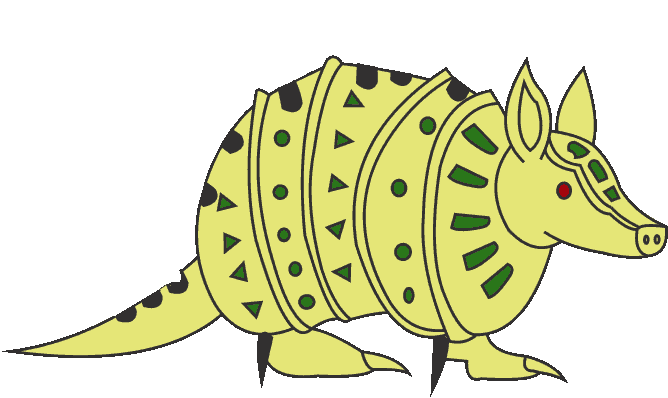
\includegraphics[height=0.2 \textheight]{Imagenes/armadilloNormal}
	\caption{Concepto de diseño del Armadillo.}
	\label{fig:armadillo}
\end{figure} 

\subsection{Encuentro:}
Enemigo del nivel tres del juego (ver apartado \ref{Nivel:Niv03}).
\subsection{Habilidades:}
\begin{itemize}
	\item Cuchillas de obsidiana (ver aparatado \ref{hab.CuchObs}).
\end{itemize}
\subsection{Patrón de ataque:}
El armadillo se moverá en un desplazamiento horizontal del punto A hacia el punto B. Durante su desplazamiento se mostrara su bloque de animación de rodar y cuando llegue a los A o B se activará su habilidad de cuchillas de obsidiana ver aparatado \ref{hab.CuchObs}). 
\subsection{Bloques de animación:}
	\begin{itemize}
		\item Animación de sacar picos.
		\item Animación rodar. 
	\end{itemize}